
\documentclass[answers,a4paper,12pt]{exam}
\usepackage{fontawesome5}
\usepackage[margin=1.5cm]{geometry}
\usepackage{relsize}
\usepackage{amssymb}
\usepackage{mathrsfs}
\usepackage{graphicx}
\usepackage[utf8]{inputenc}
\usepackage{amsmath}
\usepackage{systeme}
\graphicspath{{./images/}}
\DeclareMathOperator{\sign}{sign}
\def\dbar{{\mathchar'26\mkern-12mu d}}
\usepackage{amsthm}
\usepackage[italian]{babel}
\title{Elettronica T}
\author{Kevin Michael Frick}
\date{}
\setlength\linefillheight{.4in}
\setlength\linefillthickness{0.4pt}
\renewcommand{\solutiontitle}{\noindent\textbf{Risposta:}\enspace}
\newcommand{\bigint}{\mathop{\mathlarger{\int}}}
\newcommand{\bigoint}{\mathop{\mathlarger{\oint}}}
\newcommand{\bigiiint}{\mathop{\mathlarger{\iiint}}}
\newcommand{\bigiint}{\mathop{\mathlarger{\iint}}}
\begin{document}
\maketitle
\section*{Digitale}
\begin{questions}

\question Perché il bulk di un transistore nMOS (risp. pMOS) deve essere collegato ad una tensione minore (risp. maggiore) rispetto a quella a cui possono essere polarizzati il drain e il source?
\begin{solutionorbox}[5cm]
    Il bulk crea una giunzione di diodo con il drain e il source. 
    Ciò significa che, per evitare che ci sia passaggio di corrente, è necessario che venga tenuto ad una tensione di non conduzione.
\end{solutionorbox}

\question Disegnare lo schema elettrico di uno switch a pass transistor e giustificare la presenza contemporanea di un nMOSFET e un pMOSFET.
\begin{solutionorbox}[5cm]
\includegraphics[width=0.7\textwidth]{SwitchPassTransistor}

Il pMOSFET garantisce valore pari a $V_{DD}$ se $IN/OUT 1$, mentre il nMOSFET garantisce valore pari a $0 V$ se $IN/OUT = 0$.
\end{solutionorbox}
\question Da cosa sono causate le correnti di perdita nella logica dinamica, che difetto provocano e come viene risolto il problema?
\begin{solutionorbox}[5cm]
    Il funzionamento di una porta dinamica si appoggia all'immagazzinamento dinamico del valore di output su un condensatore.
    Se la PDN non connette a massa, l'output dovrebbe idealmente rimanere allo stato pre-caricato a $V_{DD}$ durante la fase di valutazione.
    Ciononostante, questa carica gradualmente viene persa a causa delle correnti di perdita, risultando quindi in un malfunzionamento del gate.
    La figura mostra le fonti di correnti di perdita per un basilare inverter dinamico.
    Le fonti 1 e 2 sono rispettivamente i diodi polarizzati inversamente e la perdita sotto-soglia del dispositivo nMOS di pull-down M1.
    La carica immagazzinata in $C_L$ verrà lentamente persa a causa di queste fonti di correnti di perdita, presumendo che l'output sia 0 durante la valutazione.
    La perdita di carica causa una degradazione nel livello alto. 
    I circuiti dinamici quindi richiedono che venga usata la frequenza di clock più bassa possibile, solitamente nell'ordine di qualche KHz.
    Questo rende l'uso di tecniche dinamiche poco attraente per dispositivi a basso consumo come orologi o processori con clock condizionale (nei quali non ci sono garanzie sulla frequenza minima di clock).
    Si noti che anche il dispositivo di pre-carica del pMOS contribuisce alle correnti di perdita a causa del diodo polarizzato inversamente (fonte 3) e la conduzione sotto-soglia (fonte 4).
    Fino a un certo punto la corrente di perdita del pMOS contrasta la perdita della PDN.
    Come risultato il voltaggio di output sarà configurato dal partitore resistivo composto dalla PUN e la PDN.

{\centering

\includegraphics[width=0.8\textwidth]{CorrentiPerdita.png}

}

La perdita è causata dallo stato di alta impedenza del nodo di output durante la valutazione, quando la PDN non connette a massa.
La perdita può essere contrastata riducendo l'impedenza del nodo di output durante la valutazione.
Ciò è spesso realizzato mediante un \textit{transistore bleeder} come in figura. 
L'unica funzione del bleeder - un dispositivo pseudo-nMOS di pull-up - è di compensare la carica persa a causa dei percorsi di perdita di pull-down.
Per evitare i problemi di rapporto associati con questo stile di circuito e la dissipazione di potenza statica associata, la resistenza del bleeder è resa alta o, in altre parole, il dispositivo è tenuto piccolo.
Ciò permette ai dispositivi di pull-down, più forti, di abbassare il nodo di output sotto la soglia di switching dell'inverter.
Spesso, il bleeder è implementato in una configurazione di feedback per eliminare la dissipazione statica di potenza.

{\centering

\includegraphics[width=0.8\textwidth]{SoluzioneCorrentiPerdita.png}

}

    \end{solutionorbox}
\question Cos’è la soglia logica di un inverter? Come si calcola la soglia logica di un inverter composto da un nMOS e una resistenza di pull-up?
\begin{solutionorbox}[5cm]
    La soglia logica $V_M$ è definita come il punto in cui $V_{in} = V_{out}$.
    Il suo valore può essere ottenuto analiticamente eguagliando le correnti attraverso i transistori.
    {\centering

        \includegraphics[width=0.5\textwidth]{CurvaInverter.png}

    }
    Graficamente si può osservare che le tensioni sono pari alla soglia logica quando entrambi i MOSFET sono in saturazione.
    
    \[
        \systeme*{V_{in} = \frac{K_n}{2} (V_{in} - V_{Tn})^2, V_{out} = \frac{|K_p|}{2} (V_{DD} - V_{in} - |V_{Tp}|)^2 } \implies V_M = \frac{V_{Tn} + r ( V_{DD} + V_{Tp} )}{1 + r}
    \]
    
    con $ r =\sqrt{\frac{|K_p|}{K_n}} = \sqrt{\frac{|K'_p S_p|}{K'_n S_n}}$, $K$ fattore di guadagno, $K'$ transconduttanza.
\end{solutionorbox}
\question Disegnare la struttura fisica di un transistore nMOS(risp. pMOS), indicando i tipi di drogaggi e i
diodi parassiti presenti. Inoltre indicare la formula per il calcolo della
capacità di gate.
\begin{solutionorbox}[5cm]

$C_g = C_{ox} \cdot L \cdot W = C_{ox} \cdot L^2 \cdot S$

nMOS:

{\centering

\includegraphics[width=0.8\textwidth]{nMOS.png}

}

pMOS:

{\centering

\includegraphics[width=0.8\textwidth]{pMOS.png}

}
\end{solutionorbox}

\question Disegnare un pass-transistor con la funzione di interruttore con ENABLE all’interno del contenitore sotto rappresentato, indicando per tutti i transistori necessari i collegamenti necessari.
\begin{solutionorbox}[5cm]
{\centering

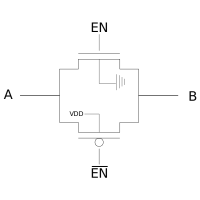
\includegraphics[width=0.5\textwidth]{PassTransistor.png}

}
\end{solutionorbox}
\question Si chiarisca l’origine della capacità di gate dei dispositivi MOS.
\begin{solutionorbox}[5cm]
La capacità di gate $C_{GC}$, o capacità di canale, dipende dalle condizioni di polarizzazione del transistor ed è composta da tre componenti: la capacità gate-source $C_{GS}$, la capacità gate-drain $C_{GD}$ e la capacità gate-bulk $C_{GB}$.


Quando il transistor è spento la capacità di gate è tra il gate e il body.
Quando il transistor è resistivo si forma un livello di inversione che si comporta come un conduttore tra source e drain. 
Di conseguenza, $C_{GB} = 0$ perché l'elettrodo del body è isolato dal gate dal canale. 
La simmetria detta che la capacità si distribuisca uniformemente tra source e drain.
Infine, nella regione di saturazione, il canale viene strozzato.
La capacità gate-drain è circa zero, così come la capacità gate-body. 
Tutta la capacità di gate è quindi tra gate e source. 
Si può approssimare e affermare che i 2/3 di tutta la capacità siano attribuibili all'accoppiamento capacitivo tra gate e source.

{\centering

\includegraphics[width=\textwidth]{CapacitaGate.png}

}


La capacità di gate-body vale $C_{GB} = \epsilon_0 \epsilon_r \frac{A}{d} = \epsilon_0 \epsilon_r \frac{WL}{t_{ox}} = C_{ox} W L$ quando il MOSFET è spento.
Le capacità gate-source e gate-drain valgono $C_{GS} = C_{GD} = C_{ox} \frac{W L}{2}$ quando il MOSFET è resistivo.
La capacità gate-source vale circa $C_{GS} = \frac{2}{3} C_{ox} W L$ quando il MOSFET è in saturazione.
\end{solutionorbox}
\question Si spieghi la differenza tra consumo di potenza statico e dinamico
\begin{solutionorbox}[5cm]
    Si ha consumo di potenza statico quando l'uscita è stabile.
    Si ha consumo di potenza dinamico quando il segnale commuta.
    La potenza dinamica è definita come $P_{DYN} = \frac{1}{2} f C V_{DD}^2$ dove $f$ è la frequenza di commutazione del sistema, $C$ è la capacità di carico pilotata dal dispositivo e $V_{DD}$ la tensione di alimentazione.
\end{solutionorbox}
\question Per quale motivo il consumo di potenza statico è di importanza crescente per le tecnologie CMOS fortemente scalate?
\begin{solutionorbox}[5cm]
    Lo scaling delle dimensioni dei MOSFET comporta anche uno scaling delle tensioni di soglia e di alimentazione. 
    Tuttavia la riduzione delle tensioni di soglia comporta che il MOSFET sia "meno spento" quando la tensione sul gate lo prevede. 
    Di conseguenza le correnti di leakage non sono più trascurabili rispetto alle correnti quando il transistore è attivo e il consumo di potenza statico diventa un fattore non trascurabile.
    Inoltre a causa dello scaling molti più transistor possono essere integrati sulla stessa area e la corrente totale di leakage è elevata.
\end{solutionorbox}
\pagebreak
\question Si tracci lo schema di un sense amplifier per DRAM e se ne discuta il funzionamento durante l’operazione di REFRESH (meno di 60 parole)
\begin{solutionorbox}[5cm]

    {\centering

\includegraphics[height=5cm]{SenseAmp}

}
    Il sense amplifier accelera la lettura e simultaneamente rinfresca il contenuto della cella, che altrimenti verrebbe distrutto dalla lettura.
    Durante l’operazione di REFRESH la tensione sulla linea BL (e BL’) viene forzata al valore logico memorizzato sul condensatore che immagazzina il valore del bit. 
    In questo modo, la perdita di informazione dovuta alle correnti parassite viene annullata.
\end{solutionorbox}
\question Perché un pass-transistor nMOS ha un transitorio di salita più lento di quello di discesa?
\begin{solutionorbox}[5cm]
    Perché il transitorio di salita avviene a $V_{GS}$ decrescente, quindi il transistore tende ad essere progressivamente meno conduttivo fino a spegnersi quando il valore della tensione in uscita raggiunge $V_{DD} - V_{Tn}$.
\end{solutionorbox}

\question Disegnare la caratteristica $I_D$ verso $V_{DS}$ di un transistore nMOS e indicare le zone di funzionamento con le relative formule per la corrente.
\begin{solutionorbox}[5cm]

    {\centering

    \includegraphics[height=7cm]{CurvaNMOS.png}

}
\end{solutionorbox}
\pagebreak
\question Disegnare uno XOR a due ingressi all’interno del contenitore sotto rappresentato, indicando per tutti i transistori necessari i collegamenti necessari, bulk compreso.
\begin{solutionorbox}[5cm]

{\centering

    \includegraphics[height=7cm]{CMOSXOR.png}

}

Il bulk, in logica CMOS, è sempre collegato al source.
\end{solutionorbox}

\question Disegnare un OR a due ingressi all'interno del contenitore sotto rappresentato, indicando tutti i collegamenti necessari, bulk compreso.
\begin{solutionorbox}[5cm]

    {\centering

    \includegraphics[height=7cm]{CMOSOR.png}

}
Il bulk, in logica CMOS, è sempre collegato al source.
\end{solutionorbox}
\pagebreak
\question Disegnare un AND a due ingressi all'interno del contenitore sotto rappresentato, indicando tutti i collegamenti necessari, bulk compreso.
\begin{solutionorbox}[5cm]

    {\centering

    \includegraphics[height=7cm]{CMOSAND.png}

}
Il bulk, in logica CMOS, è sempre collegato al source.
\end{solutionorbox}

\question Disegnare la caratteristica Ingresso-Uscita di un inverter CMOS simmetrico (nMOS e pMOS hanno la stessa resistenza di ON). Indicare lo stato dei transistori nelle diverse zone della caratteristica.
\begin{solutionorbox}[5cm]

    {
    \centering

    \includegraphics[height=7cm]{CurvaInverter.png}

}
\end{solutionorbox}
\question In quale caso si ha un deterioramento della tensione di uscita rispetto a $(0, V_{DD}$) nella logica a pass-transistor nMOS? Si faccia un esempio.
\begin{solutionorbox}[5cm]
    Si ha un deterioramento nel caso di trasferimento in uscita di valori alti ($V_{DD}$) poiché il transistor lavora in progressivo spegnimento. 
    Il potenziale del source (ovvero il terminale a potenziale minore tra i due) cresce con la carica del nodo di uscita, e determina lo spegnimento quando $V_{GS}-V_{Tn} < 0$.
\end{solutionorbox}
\question Quali sono i principali contributi di consumo di potenza nell’inverter CMOS? Da cosa dipendono e come possono essere ridotti (ove possibile)?
\begin{solutionorbox}[5cm]
Il principale consumo di potenza è quello dinamico.

Durante la commutazione dell'inverter da basso ad alto viene caricata la capacità di carico; tale capacità viene poi scaricata durante la commutazione da alto a basso. 
La potenza dinamica assorbita a causa di una doppia commutazione $(0 \rightarrow 1 \rightarrow 0)$ è pari a $P_{DYN} = C_L V_{DD}^2 / T = C_L V_{DD}^2 f_{0\rightarrow 1}$. 
La frequenza di commutazione non è necessariamente la frequenza di funzionamento del circuito: bisogna tenere conto della probabilità che l'ingresso cambi.

Durante la commutazione si crea un percorso resistivo tra la tensione di alimentazione e la massa, attraverso il quale scorre corrente e che dissipa quindi potenza.
In una doppia transizione si hanno due picchi di corrente che dissipano una potenza pari a $P_{DYN} = \bigint_{t_R}^{t_F} V_{DD} i (t) dt / T = f_{0\rightarrow 1} \frac{V_{DD} I_{peak}  (t_R + t_F)}{2}$. 
Questa corrente scorre solo se la tensione di ingresso $V_{in}$ soddisfa $V_{Tn} < V_{in} < V_{DD} - V_{Tp}$. In caso contrario uno dei transistor non è in conduzione durante la transizione.
\end{solutionorbox}
\end{questions}
\textbf{Disclaimer}:  Questo documento può contenere errori e imprecisioni che potrebbero danneggiare sistemi informatici, terminare relazioni e rapporti di lavoro, liberare le vesciche dei gatti sulla moquette e causare un conflitto termonucleare globale.  
Procedere con cautela.

Questo documento è rilasciato sotto licenza CC-BY-SA 4.0. \faCreativeCommons\ \faCreativeCommonsBy\ \faCreativeCommonsSa
\end{document}
